\documentclass[tikz,border=8pt]{standalone}
\usetikzlibrary{arrows.meta,positioning,calc}
\begin{document}
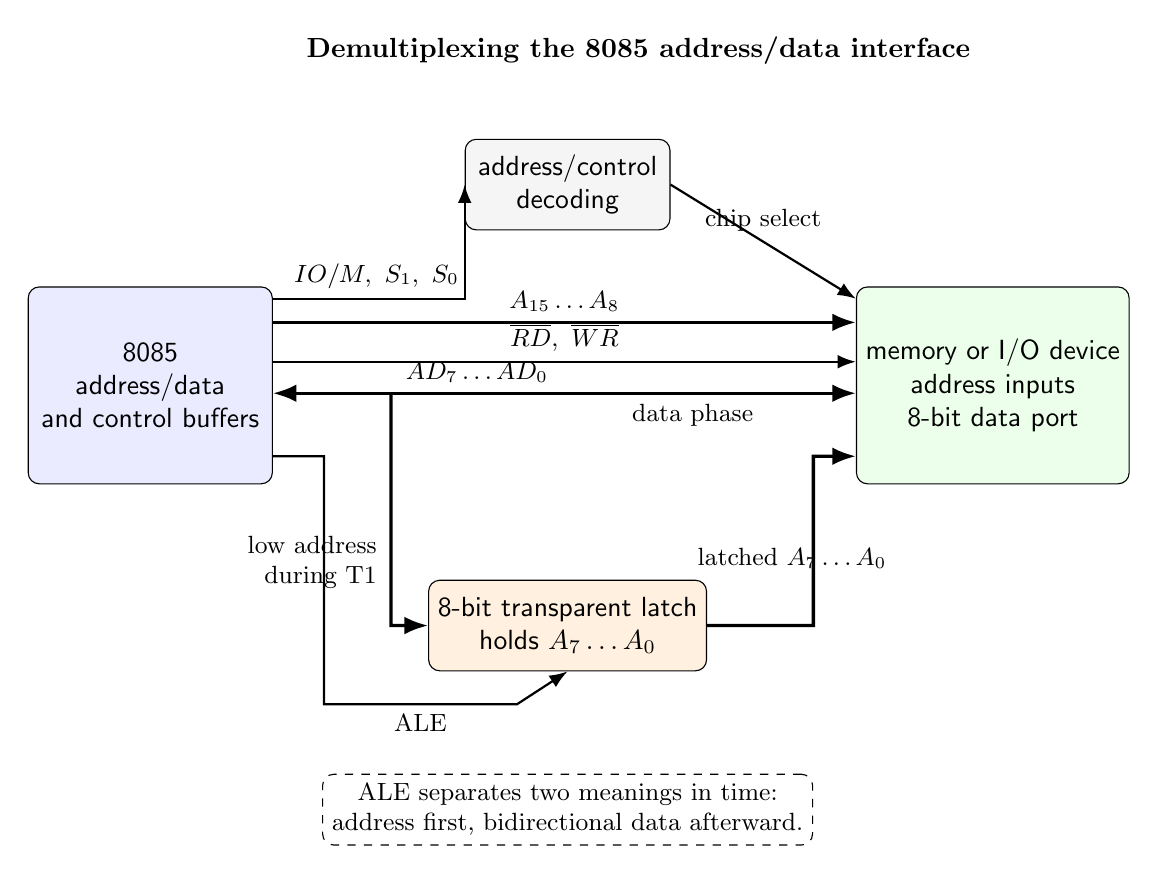
\begin{tikzpicture}[
  font=\sffamily,
  >=Latex,
  block/.style={draw,rounded corners,minimum width=3.1cm,minimum height=2.5cm,align=center},
  smallblock/.style={draw,rounded corners,minimum width=2.6cm,minimum height=1.15cm,align=center},
  bus/.style={line width=1.2pt,-{Latex[length=3mm]}},
  bibs/.style={{Latex[length=3mm]}-{Latex[length=3mm]},line width=1.2pt},
  ctrl/.style={->,thick}
]
\node[font=\bfseries] at (6.2,4.25) {Demultiplexing the 8085 address/data interface};
\node[block,fill=blue!8] (cpu) at (0,0) {8085\\address/data\\and control buffers};
\node[smallblock,fill=orange!12] (latch) at (5.3,-3.05) {8-bit transparent latch\\holds $A_7\ldots A_0$};
\node[smallblock,fill=gray!8] (decode) at (5.3,2.55) {address/control\\decoding};
\node[block,fill=green!8] (mem) at (10.7,0) {memory or I/O device\\address inputs\\8-bit data port};

\draw[bus] ([yshift=8mm]cpu.east) -- node[above,font=\small] {$A_{15}\ldots A_8$} ([yshift=8mm]mem.west);
\draw[bibs] ([yshift=-1mm]cpu.east) -- node[above,font=\small,pos=.35] {$AD_7\ldots AD_0$} node[below,font=\small,pos=.72] {data phase} ([yshift=-1mm]mem.west);
\draw[bus] ([yshift=-1mm,xshift=15mm]cpu.east) -- ++(0,-2.95) -- (latch.west);
\node[font=\small,align=right,anchor=east] at (3.0,-2.25) {low address\\during T1};
\draw[bus] (latch.east) -- ++(1.35,0) -- ++(0,2.15) -- ([yshift=-9mm]mem.west);
\node[font=\small] at (8.15,-2.20) {latched $A_7\ldots A_0$};

\draw[ctrl] ([yshift=-9mm]cpu.east) -- ++(0.65,0) -- ++(0,-3.15) -- node[below,font=\small] {ALE} ++(2.45,0) -- (latch.south);
\draw[ctrl] ([yshift=11mm]cpu.east) -| node[pos=.27,above,font=\small] {$IO/M,\ S_1,\ S_0$} (decode.west);
\draw[ctrl] (decode.east) -- node[above,font=\small] {chip select} ([yshift=11mm]mem.west);
\draw[ctrl] ([yshift=3mm]cpu.east) -- node[above,font=\small] {$\overline{RD},\ \overline{WR}$} ([yshift=3mm]mem.west);

\node[draw,dashed,rounded corners,align=center,below=13mm of latch,font=\small] {ALE separates two meanings in time:\\address first, bidirectional data afterward.};
\end{tikzpicture}
\end{document}
